\chapter{Various}

\section{Structs}
\kactlimport{Fraction.h}

\section{Skills}
\kactlimport{Random.h}
\kactlimport{Getline.h}
\kactlimport{Stress.h}

\section{Some primes for NTT, hashing}
$998244353 = 119 \times 2^{23} + 1$, Primitive root = 3 \\
$985661441 = 235 \times 2^{22} + 1$, Primitive root = 3 \\
$1012924417 = 483 \times 2^{21} + 1$, Primitive root = 5

\section{Tricks}
\kactlimport{BitsOperation.h}
\kactlimport{FloorLoop.h}

\section{Optimization}
\kactlimport{FastIO.h}
\kactlimport{FastMod.h}

\section{Dynamic programming}
\kactlimport{KnuthDP.h}
\kactlimport{DivideAndConquerDP.h}

\section{Graph Matching Application about cubic time}
\begin{itemize}
    \setlength\itemsep{0.1em}
    \item \textbf{Game on a Graph}: There is a token on vertex $s$. Each player moves the token to an adjacent vertex on their turn and loses if they cannot move.\\
    There exists a maximum matching that does not include $s$ $\leftrightarrow$ the second player to move wins.
    \item \textbf{Chinese Postman Problem}: The problem of finding the minimum weight circuit that visits every edge. Revisiting node and edges is allowed. \\
    Run Floyd's algorithm, then pair up odd-degree vertices to find the minimum weight matching (there are an even number of odd-degree vertices).
    \item \textbf{Unweighted Edge Cover}: The problem of finding the smallest set of edges (minimum cardinality/weight) that covers all vertices.\\
    $\vert V\vert - \vert M\vert$, no path of length 3, composed of several star graphs.
    \item \textbf{Weighted Edge Cover}: $sum_{v \in V}(w(v)) - sum_{(u,v) \in M}(w(u) + w(v) - d(u,v))$, where $w(x)$ is the minimum weight of an edge adjacent to $x$.
    \item \textbf{NEERC'18 B}: A problem where each machine must be operated by two workers, and each worker can operate at most one machine. Maximize the number of machines which works. \\
    Create two vertices for each machine and connect them with an edge, the solution is $\vert M\vert - \vert\text{machines}\vert$. It's good to consider that each contributes 1/2 to the solution.
    \item \textbf{Min Disjoint Cycle Cover}: The problem of finding a set of cycles of length 3 or more that covers all vertices without overlap.\\
    Each vertex must be matched with two distinct edges, and some edges must be matched with both endpoints, so we can think of flow, but flow is not possible since only one unit of flow can be sent through an edge with capacity 2.\\
    Copy each vertex and edge into two ($(v, v')$, $(e_{i,u},e_{i,v})$). For every edge $e=(u,v)$, create a weighted edge of weight $w$ connecting $e_u$ and $e_v$ (like NEERC18), and create weight 0 edges connecting $(u,e_{i,u}), (u',e_{i,u}), (v,e_{i,v}), (v',e_{i,v})$. The existence of a perfect matching $\leftrightarrow$ existence of a Disjoint Cycle Cover. Find the maximum weight matching and then subtract the matching from the sum of all edge weights.
    \item \textbf{Two Matching}: The problem of finding the maximum weight matching where each vertex is adjacent to at most two edges.\\
      Each component must become a single vertex/path/cycle. Create a weight 0 edge for every distinct pair of vertices, and a weight 0 edge $(v,v')$ turns it into a Disjoint Cycle Cover problem. Components with only one vertex are self-loops, and it's convenient to think of path-shaped components as having their endpoints connected.
    \item \textbf{Parith Shortest Simple Path}: Without loss of generality, let's say we're looking for a path of even length (the same method applies for odd length). We create a copy $G'$ of graph $G$, but instead of connecting opposite sides, for every edge $e = \{u, v\}$, we connect $G(u) \leftrightarrow G(v)$ and $G'(u) \leftrightarrow G'(v)$. Finally, for every vertex $v \in V$, we connect the vertices $G(v) \leftrightarrow G'(v)$. In this graph, if we find a perfect matching, the vertices of the original graph $G$ will either be covered by the edges connecting $G(v) \leftrightarrow G'(v)$ or be part of even cycles that alternate between $G$ and $G'$. \\
      Now, let's remove $G(s), G'(t)$ and find a perfect matching. Start from the matched vertex $v$ of $G'(s)$, switch sides, and continue following the matched vertices in the same manner. During this process, we will never encounter edges connecting $G(v) \leftrightarrow G'(v)$. This process will not end until it reaches $t$, and it is guaranteed to terminate. Listing the vertices we encounter along the path gives us a path with an even number of edges. This way, we can confirm the existence of a Parity shortest path between $s$ and $t$. To find the shortest path, set the weight of the edges connecting $G(v) \leftrightarrow G'(v)$ to 0, and use the original weights for the other edges.
    \item \textbf{Planar Graph Max Cut}: Given a graph, let's divide the set of vertices into two non-empty subsets (S, V\S). The goal is to maximize the number of edges between the two subsets. (In contrast, Global Min Cut minimizes this number.) \\
The case where the answer to the Global Min Cut is 0 is when the graph is not connected, but the case where the answer to the Global Max Cut is the total number of edges is when the graph is bipartite. In other words, Max Cut is the problem of removing the minimum number of edges to make the graph bipartite.\\
What properties does a Planar Graph have if it's bipartite? Planar graphs have a very useful concept called the Dual. The Dual of a planar graph has the same set of edges, but the set of vertices is replaced with faces. Here, each face is a cycle, and since a bipartite graph has no odd cycles, each cycle is adjacent to an even number of edges. In other words, if a Planar Graph is bipartite, then every vertex in its Dual has even degree. Another way to say this is that an Euler circuit exists.\\
At this point, the problem looks almost identical to the Chinese postperson Problem, but there is a slight difference. In the Chinese postperson problem, existing edges are duplicated, while here, the operation is to compress the edge separating two faces, effectively merging them. Even if we think of it as an operation that merges two vertices, by finding a minimum weight matching for the Dual graph in the same way as the postperson problem and then combining the edges that entered the matching, we have a possible solution. If two vertices of degrees x and y are merged, the new vertex has degree $x+y-2$, and this operation results in two odd-degree vertices matched together being combined into one vertex. Now we need to show that this is the optimal solution, and we can do so using the same proof technique used in problem 1.
\end{itemize}

\section{Something Else}
Suurballe's algorithm: finding two disjoint paths in a nonnegatively-weighted directed graph so that both paths connect the same pair of vertices and have minimum total length.

1. Find the shortest path tree T rooted at node s by running Dijkstra's algorithm. This tree contains for every vertex u, a shortest path from s to u. Let $P_1$ be the shortest cost path from s to t. The edges in T are called tree edges and the remaining edges (the edges missing from figure C) are called non-tree edges.
2. Modify the cost of each edge in the graph by replacing the cost $w(u,v)$ of every edge $(u,v)$ by $w'(u, v) = w(u, v) - d(s, v) + d(s, u)$. According to the resulting modified cost function, all tree edges have a cost of 0, and non-tree edges have a non-negative cost.
3. Create a residual graph $G_t$ formed from $G$ by removing the edges of $G$ on path $P_1$ that are directed into s and then reverse the direction of the zero length edges along path $P_1$.
4. Find the shortest path $P_2$ in the residual graph $G_t$ by running Dijkstra's algorithm.
5. Discard the reversed edges of $P_2$ from both paths. The remaining edges of $P_1$ and $P_2$ form a subgraph with two outgoing edges at s, two incoming edges at t, and one incoming and one outgoing edge at each remaining vertex. Therefore, this subgraph consists of two edge-disjoint paths from s to t and possibly some additional (zero-length) cycles. Return the two disjoint paths from the subgraph.

\section{Dominator Tree}
\begin{minipage}{90mm}
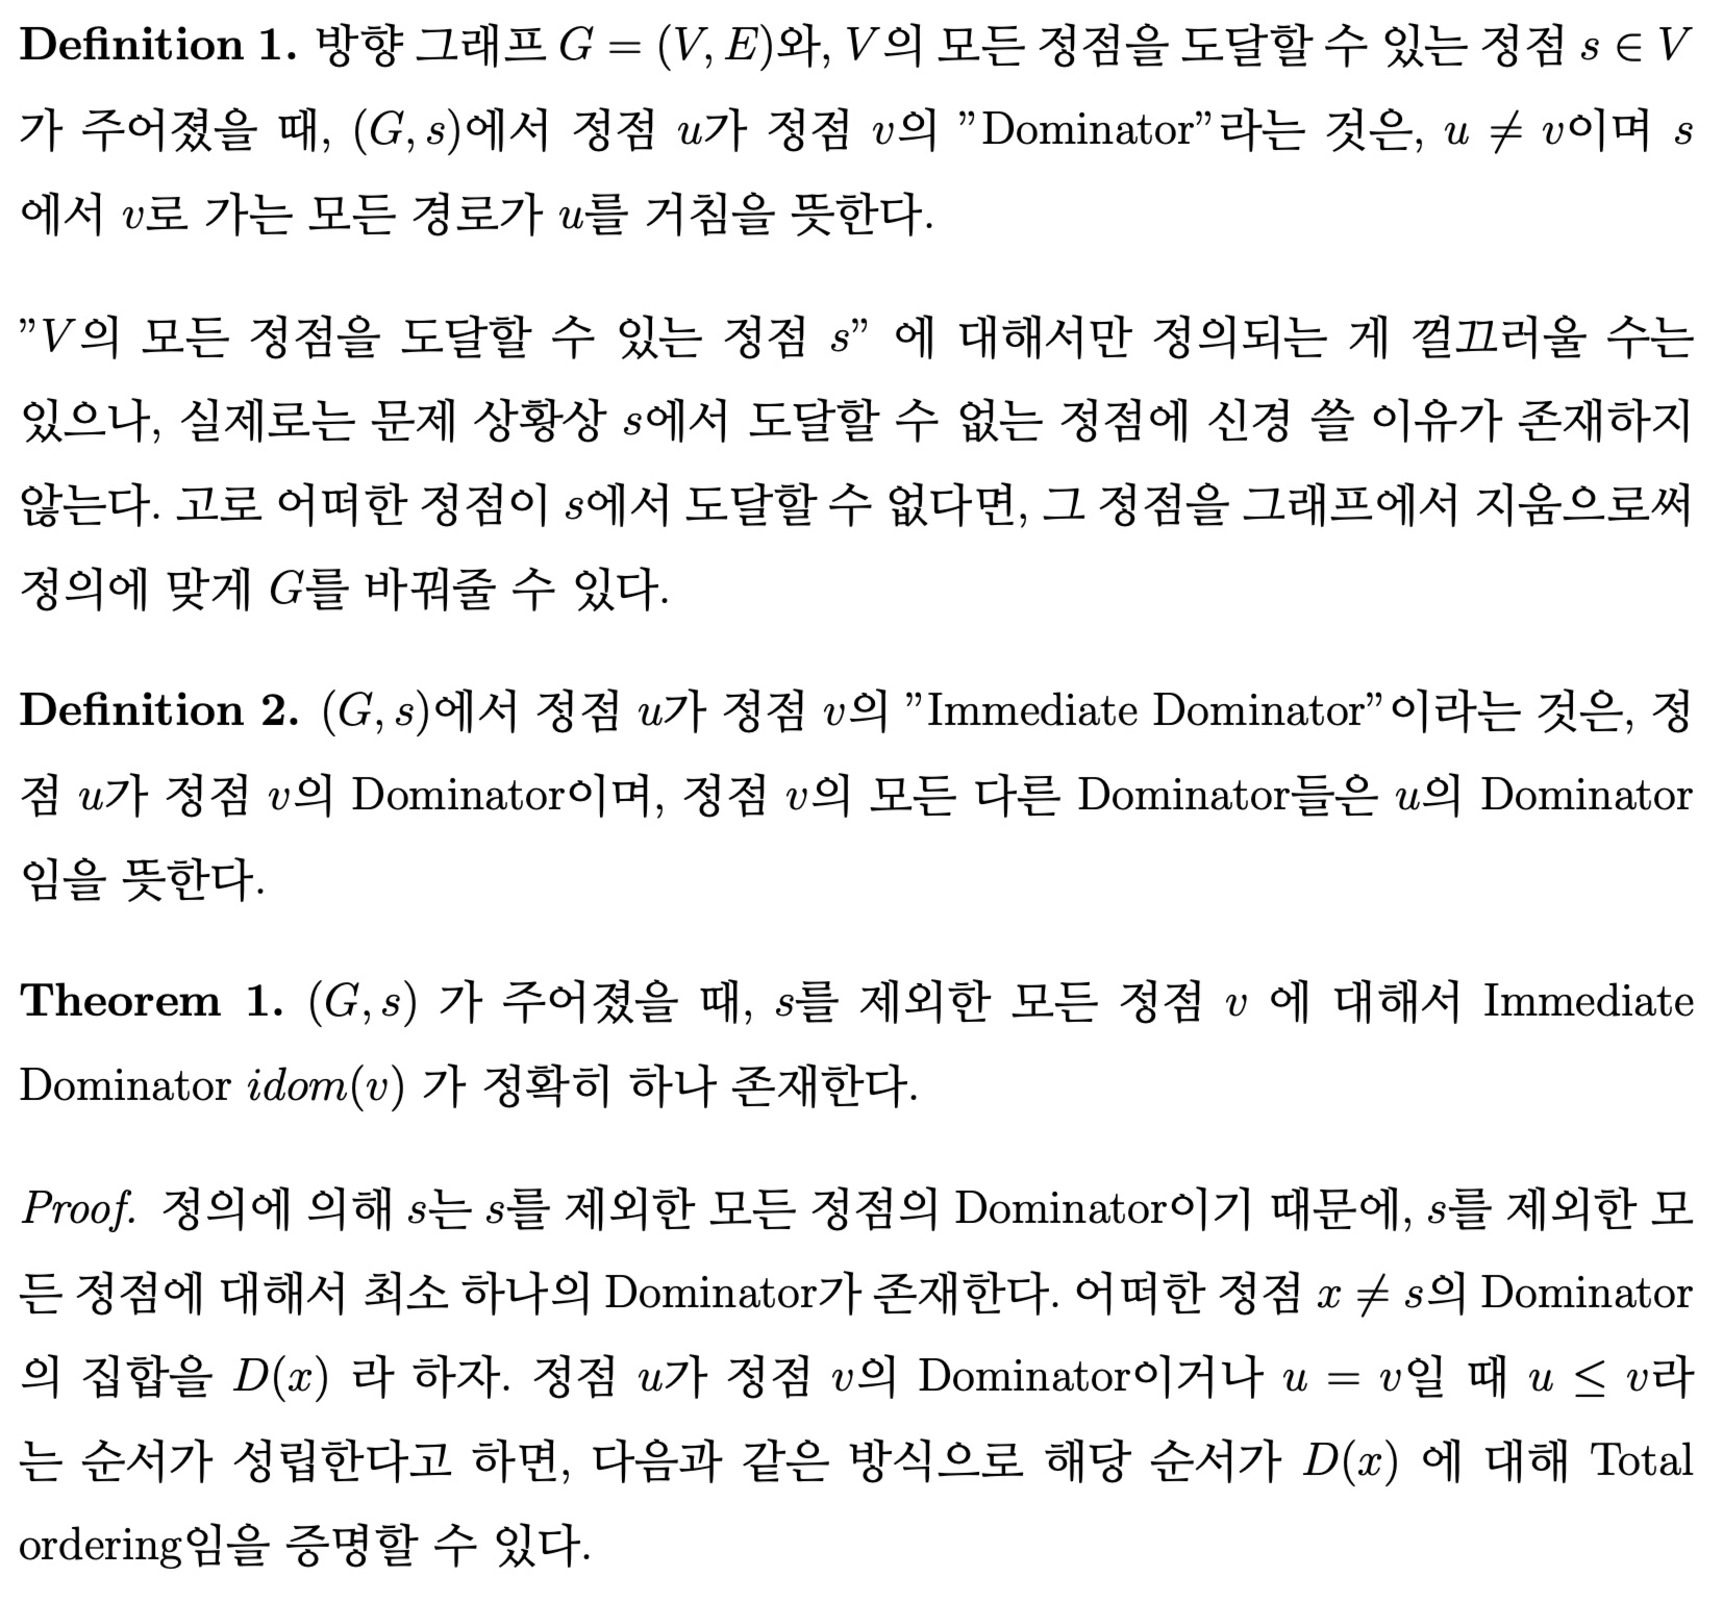
\includegraphics[width=\textwidth]{content/various/d1}
\end{minipage}
\begin{minipage}{90mm}
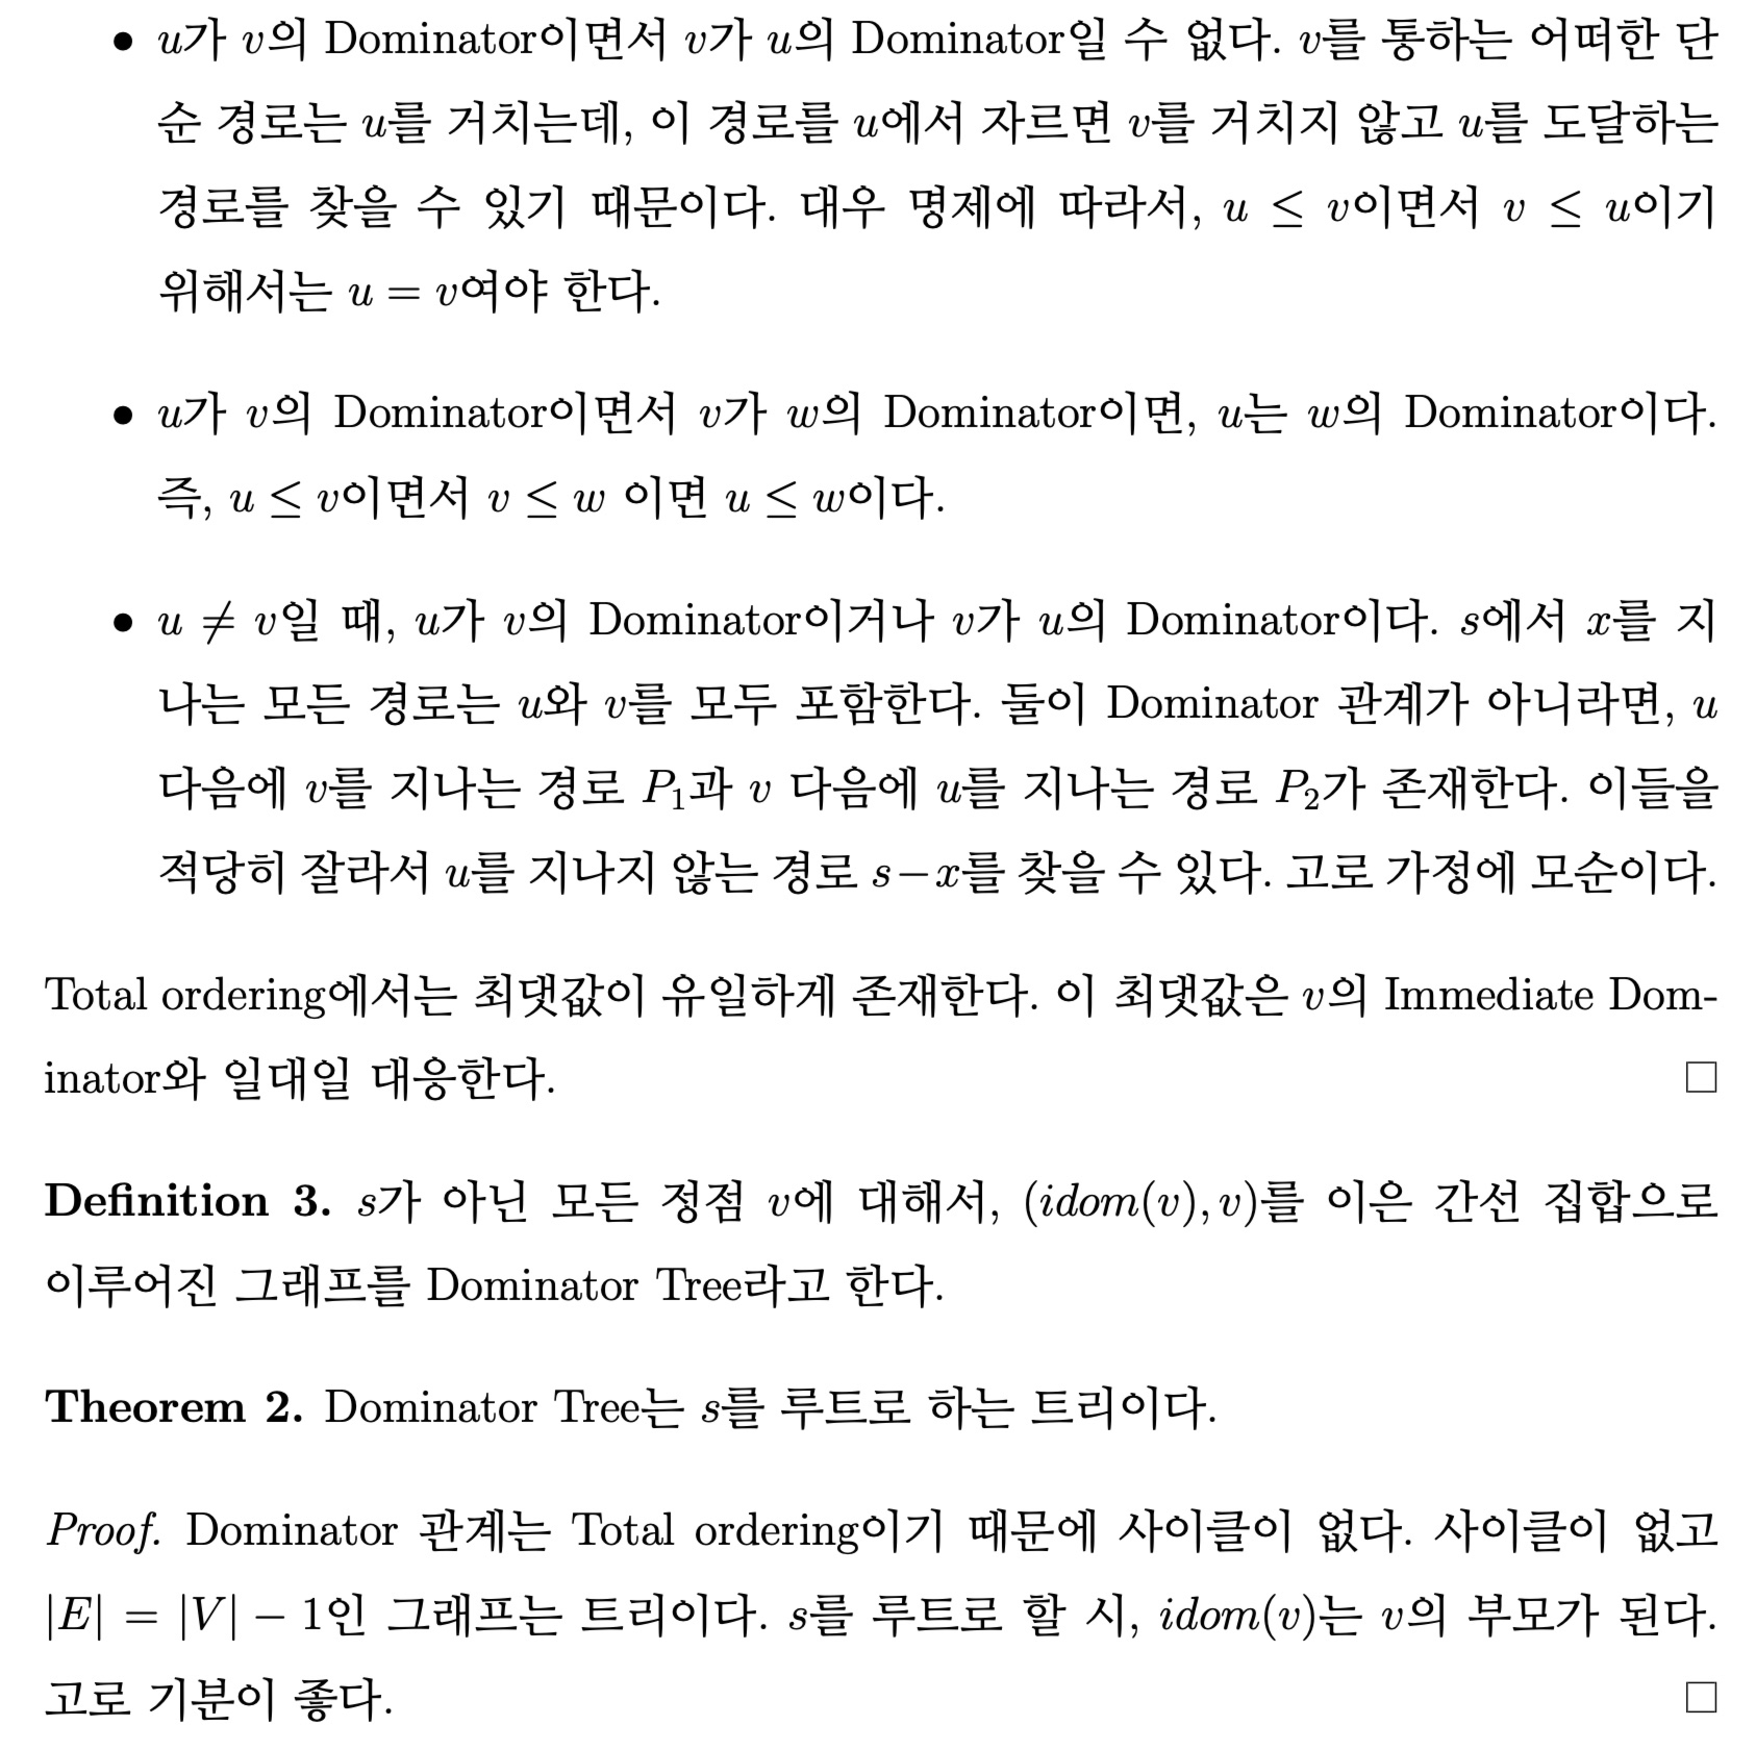
\includegraphics[width=\textwidth]{content/various/d2}
\end{minipage}

\section{Continue}
\begin{minipage}{90mm}
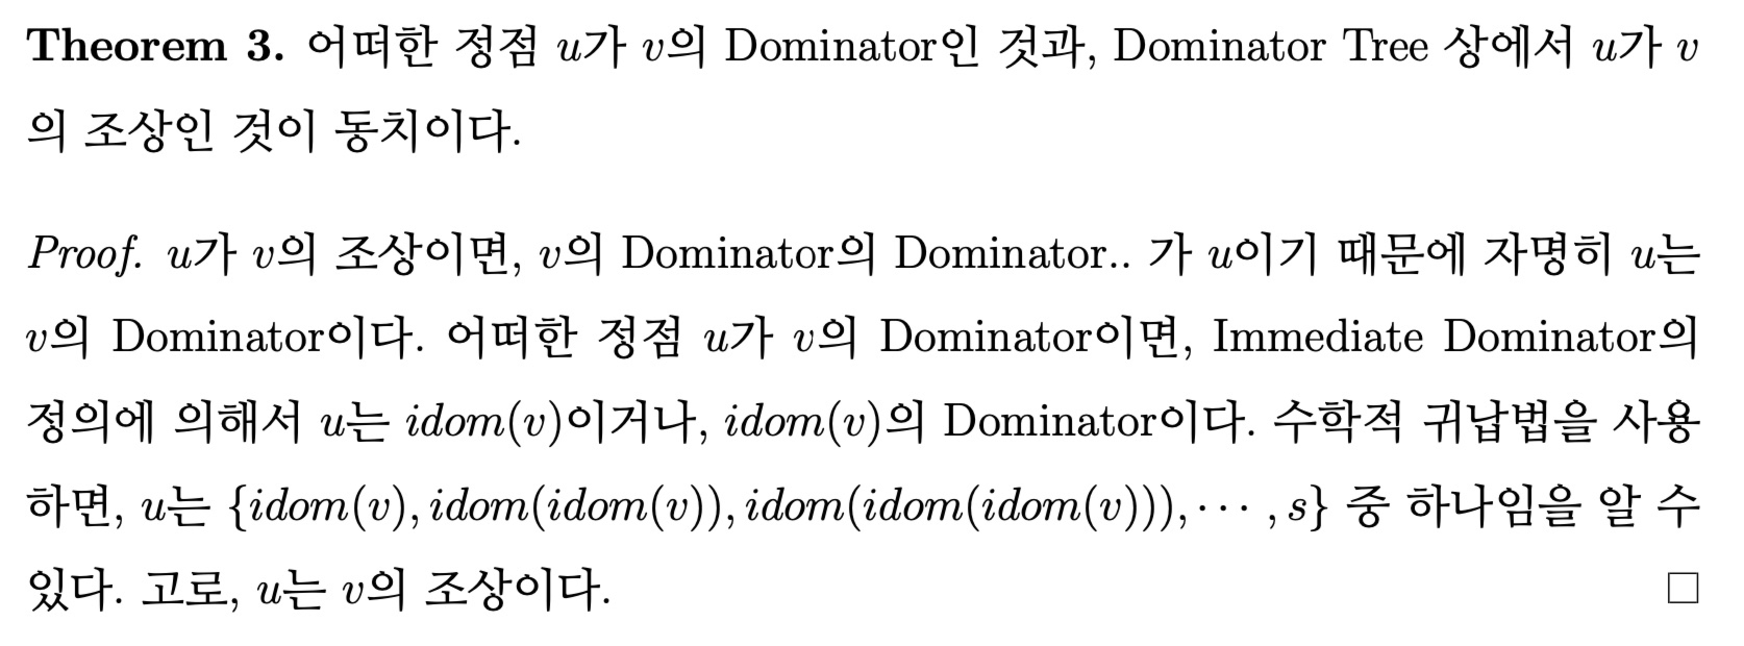
\includegraphics[width=\textwidth]{content/various/d3}
\end{minipage}
\begin{minipage}{90mm}
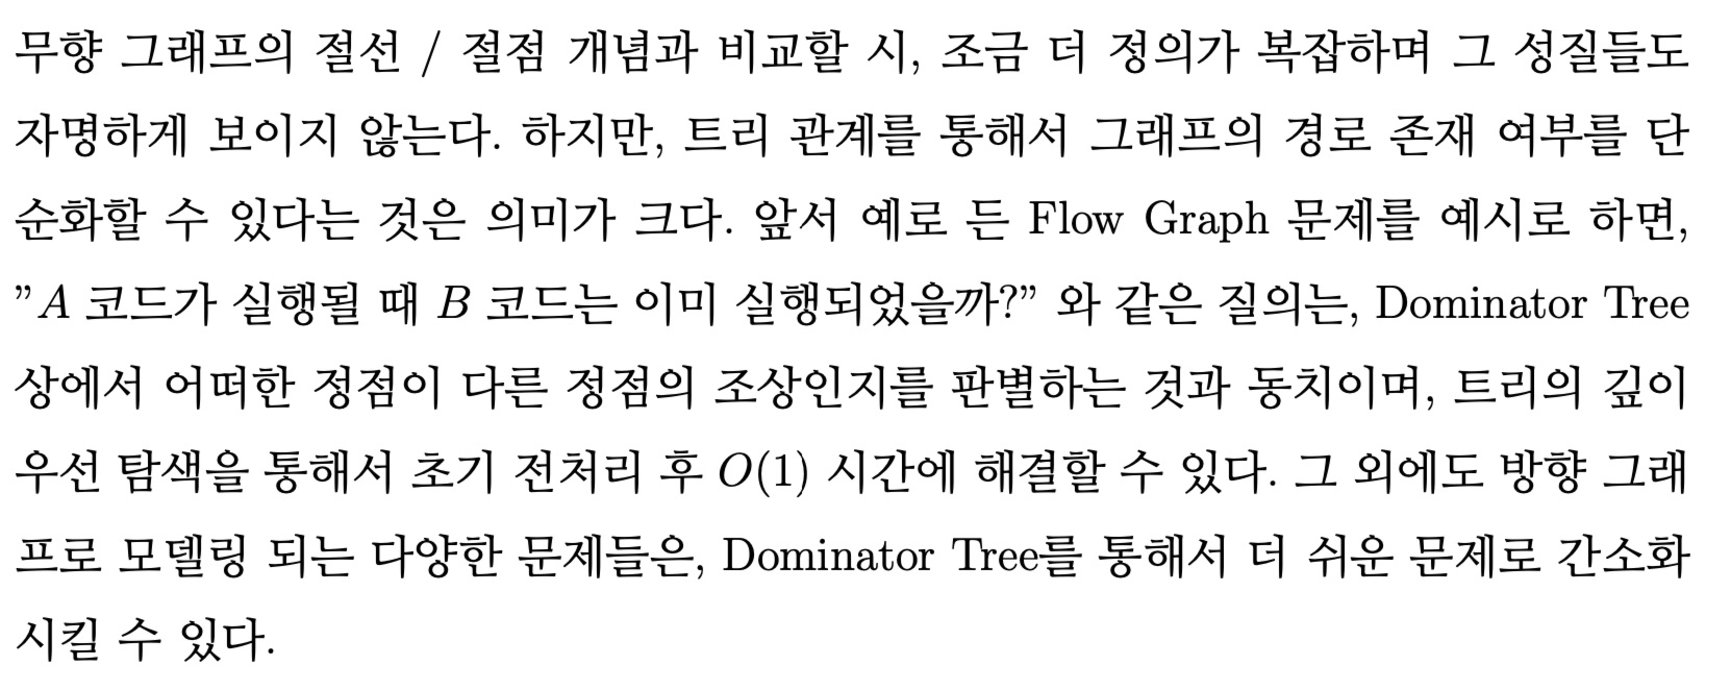
\includegraphics[width=\textwidth]{content/various/d4}
\end{minipage}

\section{Tourist}
\begin{minipage}{90mm}

\includegraphics[width=\textwidth]{content/various/tourist}
\end{minipage}

\section{Tourist}
\begin{minipage}{90mm}

\includegraphics[width=\textwidth]{content/various/tourist}
\end{minipage}
